\documentclass[11pt,oneside]{article}
\usepackage[a4paper,top=2.6cm,bottom=2.8cm,left=2.4cm,right=2.4cm,headheight=16pt]{geometry}
\usepackage[utf8]{inputenc}
\usepackage[T1]{fontenc}
\usepackage[spanish,es-tabla]{babel}
\usepackage{xcolor}
\usepackage{titlesec}
\usepackage{fancyhdr}
\usepackage{booktabs}
\usepackage{array}
\usepackage{colortbl}
\makeatletter
\@ifundefined{insert@pcolumn}{\let\insert@pcolumn\insert@column}{}
\makeatother
\usepackage[most]{tcolorbox}
\usepackage{tikz}
\usepackage{enumitem}
\usepackage{amsmath,amssymb}
\usepackage{graphicx}
\usepackage{caption}
\usepackage{listings}
\usepackage{hyperref}
\usepackage{xurl}
\usepackage{setspace}

\definecolor{primnavy}{HTML}{0B2545}
\definecolor{deepteal}{HTML}{0F5C57}
\definecolor{accentgold}{HTML}{B4771F}
\definecolor{softgray}{HTML}{F4F6F8}
\definecolor{midgray}{HTML}{6B7280}
\definecolor{linegray}{HTML}{D9DEE3}
\definecolor{rowblue}{HTML}{E8EEF4}

\titleformat{\section}{\normalfont\Large\bfseries\color{primnavy}}{\thesection}{0.6em}{}[{\color{accentgold}\titlerule[1.1pt]}]
\titleformat{\subsection}{\normalfont\large\bfseries\color{deepteal}}{\thesubsection}{0.6em}{}
\titlespacing*{\section}{0pt}{20pt}{9pt}
\titlespacing*{\subsection}{0pt}{14pt}{7pt}

\pagestyle{fancy}
\fancyhf{}
\renewcommand{\headrulewidth}{0.4pt}
\renewcommand{\footrulewidth}{0pt}
\fancyhead[L]{\small\color{midgray}Actividad 03 --- Algoritmos de enjambre}
\fancyhead[R]{\small\color{midgray}Luna Luque, P.}
\fancyfoot[C]{\small\color{midgray}Universidad Nacional del Altiplano \textbullet\ Ingenieria de Sistemas}
\fancyfoot[R]{\small\color{midgray}\thepage}
\setlength{\parindent}{0pt}
\setlength{\parskip}{6pt}
\onehalfspacing
\hypersetup{colorlinks=true,linkcolor=primnavy,citecolor=deepteal,urlcolor=deepteal,
  pdftitle={Algoritmos de enjambre aplicados al aprendizaje automatico},
  pdfauthor={Paolo Boris Luna Luque}}

\newtcolorbox{cajadef}[1][]{enhanced,colback=white,colframe=primnavy,boxrule=0.7pt,arc=1.5pt,left=8pt,right=8pt,top=7pt,bottom=7pt,title={\textbf{\textcolor{white}{#1}}},colbacktitle=primnavy,coltitle=white,fonttitle=\bfseries\small,attach boxed title to top left={xshift=8pt,yshift=-2mm},boxed title style={boxrule=0pt,arc=1.5pt}}
\newtcolorbox{cajateal}[1][]{enhanced,colback=softgray,colframe=deepteal,boxrule=0.6pt,arc=1.5pt,left=8pt,right=8pt,top=7pt,bottom=7pt,title={\textbf{\textcolor{white}{#1}}},colbacktitle=deepteal,coltitle=white,fonttitle=\bfseries\small,attach boxed title to top left={xshift=8pt,yshift=-2mm},boxed title style={boxrule=0pt,arc=1.5pt}}
\newtcolorbox{cajagold}[1][]{enhanced,colback=softgray,colframe=accentgold,boxrule=0.6pt,arc=1.5pt,left=8pt,right=8pt,top=7pt,bottom=7pt,title={\textbf{\textcolor{white}{#1}}},colbacktitle=accentgold,coltitle=white,fonttitle=\bfseries\small,attach boxed title to top left={xshift=8pt,yshift=-2mm},boxed title style={boxrule=0pt,arc=1.5pt}}
\newtcolorbox{cajarepo}{enhanced,colback=softgray,colframe=deepteal,boxrule=0.7pt,arc=2pt,left=10pt,right=10pt,top=8pt,bottom=8pt,title={\textbf{\textcolor{white}{Repositorio GitHub}}},colbacktitle=deepteal,coltitle=white,fonttitle=\bfseries\small,attach boxed title to top left={xshift=8pt,yshift=-2mm},boxed title style={boxrule=0pt,arc=1.5pt}}

\lstset{backgroundcolor=\color{softgray},basicstyle=\ttfamily\footnotesize\color{black},commentstyle=\color{deepteal},keywordstyle=\color{primnavy}\bfseries,numbers=left,numberstyle=\tiny\color{midgray},frame=single,rulecolor=\color{linegray},breaklines=true,showstringspaces=false,xleftmargin=1.2em,framexleftmargin=1.2em,tabsize=2}
\captionsetup{font=small,labelfont={bf,color=primnavy},skip=6pt}

\begin{document}
\begin{titlepage}
\begin{tikzpicture}[remember picture, overlay]
  \fill[primnavy] (current page.north west) rectangle ([yshift=-0.28cm]current page.north east);
  \fill[accentgold] ([yshift=-0.28cm]current page.north west) rectangle ([yshift=-0.42cm]current page.north east);
  \fill[deepteal] (current page.south west) rectangle ([yshift=0.28cm]current page.south east);
  \fill[accentgold] ([yshift=0.28cm]current page.south west) rectangle ([yshift=0.42cm]current page.south east);
\end{tikzpicture}
\vspace{0.35cm}
\begin{center}

\includegraphics[height=3.05cm]{../figures/escudo-unap.png}\\[0.35cm]
{\bfseries\color{primnavy} UNIVERSIDAD NACIONAL DEL ALTIPLANO}\\[0.12cm]
{\small\bfseries\color{deepteal} FACULTAD DE INGENIERIA MECANICA ELECTRICA, ELECTRONICA Y DE SISTEMAS}\\[0.04cm]
{\small\bfseries\color{deepteal}(FIMEES)}\\[0.08cm]
{\small\color{midgray} Escuela Profesional de Ingenieria de Sistemas}\\[0.45cm]
\begin{tikzpicture}\draw[accentgold, line width=1.15pt] (0,0) -- (10.2,0);\end{tikzpicture}\\[0.45cm]
{\color{midgray}\small\bfseries ACTIVIDAD 03 \textbullet\ APRENDIZAJE DE MAQUINA}\\[0.55cm]
{\LARGE\bfseries\color{primnavy} Algoritmos de enjambre}\\[0.12cm]
{\Large\bfseries\color{deepteal} aplicados al aprendizaje automatico}\\[0.38cm]
{\normalsize\itshape\color{midgray} Feature selection $\cdot$ ajuste de hiperparametros\\
entrenamiento de redes sin backpropagation $\cdot$ clustering}\\[0.45cm]
\begin{tikzpicture}\draw[accentgold, line width=1pt] (0,0) -- (9,0);\end{tikzpicture}\\[0.5cm]
\begin{tabular}{@{}rl@{}}
\textbf{\color{primnavy}Curso:} & Aprendizaje de Maquina --- IX ciclo, grupo B \\[3pt]
\textbf{\color{primnavy}Docente:} & Mayenka Fernandez Chambi \\[3pt]
\textbf{\color{primnavy}Presentado por:} & Paolo Boris Luna Luque \\[3pt]
\textbf{\color{primnavy}Facultad:} & FIMEES \\[3pt]
\textbf{\color{primnavy}Escuela Profesional:} & Ingenieria de Sistemas \\
\end{tabular}\\[0.7cm]
\begin{tcolorbox}[colback=softgray,colframe=deepteal,boxrule=0.5pt,arc=2pt,left=10pt,right=10pt,top=7pt,bottom=7pt,width=0.88\textwidth]
\centering
{\small\bfseries\color{deepteal} Repositorio de codigo}\\[2pt]
\url{https://github.com/paololuna-luw/algoritmos-enjambre}\\[2pt]
{\scriptsize\color{midgray}incluye README, codigo fuente, figuras y este informe}
\end{tcolorbox}
\vfill
{\bfseries\color{primnavy} Puno, Peru --- Septiembre de 2026}
\end{center}
\end{titlepage}

\tableofcontents
\newpage

\section{Introduccion}
Los algoritmos de enjambre resuelven problemas de optimizacion con poblaciones de agentes simples que cooperan. En aprendizaje automatico esa idea aparece de forma natural: elegir variables, ajustar hiperparametros, hallar pesos de una red o colocar centroides son problemas de busqueda.

Este informe desarrolla cuatro ejemplos ejecutables. En cada uno se explicita el ciclo que pide la actividad.

\begin{cajadef}[Ciclo del enjambre --- presente en los cuatro ejemplos]
\begin{enumerate}[leftmargin=1.4em,itemsep=2pt]
  \item Representacion de la particula (o fuente de alimento).
  \item Inicializacion del enjambre.
  \item Funcion de aptitud.
  \item Comportamiento del agente.
  \item Evolucion.
  \item Criterio de finalizacion.
\end{enumerate}
\end{cajadef}

Se implementaron \textbf{Artificial Bee Colony} (ABC) en representacion binaria para seleccion de caracteristicas y \textbf{Particle Swarm Optimization} (PSO) para las demas tareas, ambos desde cero en Python (NumPy + scikit-learn).

\begin{cajarepo}
Codigo, figuras y README:\\
\url{https://github.com/paololuna-luw/algoritmos-enjambre}
\end{cajarepo}

\section{Marco breve de los algoritmos}
\subsection{Artificial Bee Colony (ABC)}
ABC modela tres roles: abejas empleadas, observadoras y exploradoras. Cada fuente de alimento es una solucion candidata. Las empleadas explotan vecindarios; las observadoras eligen fuentes con probabilidad proporcional a la aptitud; las exploradoras abandonan fuentes estancadas y vuelven a muestrear el espacio.

\subsection{Particle Swarm Optimization (PSO)}
Cada particula $i$ tiene posicion $\mathbf{x}_i$ y velocidad $\mathbf{v}_i$. Recuerda su mejor posicion personal $\mathbf{p}_i$ y conoce la mejor global $\mathbf{g}$:
\begin{align}
\mathbf{v}_i^{t+1}
&= w\,\mathbf{v}_i^{t}
+ c_1 r_1 (\mathbf{p}_i-\mathbf{x}_i^{t})
+ c_2 r_2 (\mathbf{g}-\mathbf{x}_i^{t}), \\
\mathbf{x}_i^{t+1}
&= \mathrm{clip}\bigl(\mathbf{x}_i^{t}+\mathbf{v}_i^{t+1},\;
\mathbf{x}_{\min},\,\mathbf{x}_{\max}\bigr).
\end{align}
$w$ es la inercia, $c_1$ la memoria cognitiva y $c_2$ la social.

\section{Feature selection con ABC}
\subsection{Problema}
Dado un conjunto de $d$ caracteristicas, se busca una mascara binaria $\mathbf{m}\in\{0,1\}^d$ que maximice la exactitud de un clasificador y reduzca la cardinalidad. Problema principal: \emph{Breast Cancer Wisconsin} ($n=569$, $d=30$). Corroboracion: \emph{Wine} ($n=178$, $d=13$).

\subsection{Ciclo del enjambre}
\begin{cajateal}[Ciclo ABC --- feature selection]
\textbf{Representacion.} Fuente de alimento $=$ vector binario de longitud $d$.\\[3pt]
\textbf{Inicializacion.} $S=8$ fuentes aleatorias en $\{0,1\}^d$, con al menos un bit activo.\\[3pt]
\textbf{Aptitud.} Wrapper con regresion logistica y CV estratificada de 3 pliegues:
\[f(\mathbf{m})=\mathrm{Acc}_{CV}(\mathbf{m})-\lambda\,\frac{\|\mathbf{m}\|_0}{d},\qquad\lambda=0.012.\]
\textbf{Comportamiento.} La vecindad voltea un bit. Observadoras con ruleta. Exploradora si no hay mejora en $\mathrm{limit}=4$ ciclos.\\[3pt]
\textbf{Parada.} 8 ciclos. Se conserva la mejor fuente global.
\end{cajateal}

\subsection{Protocolo}
Estandarizacion $z$-score. \texttt{LogisticRegression(solver=liblinear)}. Semilla $42$. Baselines: vector completo y \texttt{SelectKBest} con la misma cardinalidad.

\subsection{Resultados}
ABC redujo Breast Cancer de 30 a 13 variables y subio la exactitud de $0.975$ a $0.981$. SelectKBest con $k=13$ quedo en $0.949$. En Wine paso de 13 a 6 variables, con $0.983$ frente a $0.978$ usando todas.

\begin{table}[ht]
\centering
\caption{Seleccion de caracteristicas con ABC.}
\begin{tabular}{lccc}
\toprule
\rowcolor{rowblue}
\textbf{Dataset} & $|\mathbf{m}|$ / $d$ & Acc.\ todas & Acc.\ ABC \\
\midrule
Breast Cancer & 13 / 30 & 0.975 & \textbf{0.981} \\
Wine          & 6 / 13  & 0.978 & \textbf{0.983} \\
\bottomrule
\end{tabular}
\end{table}

\begin{figure}[ht]\centering
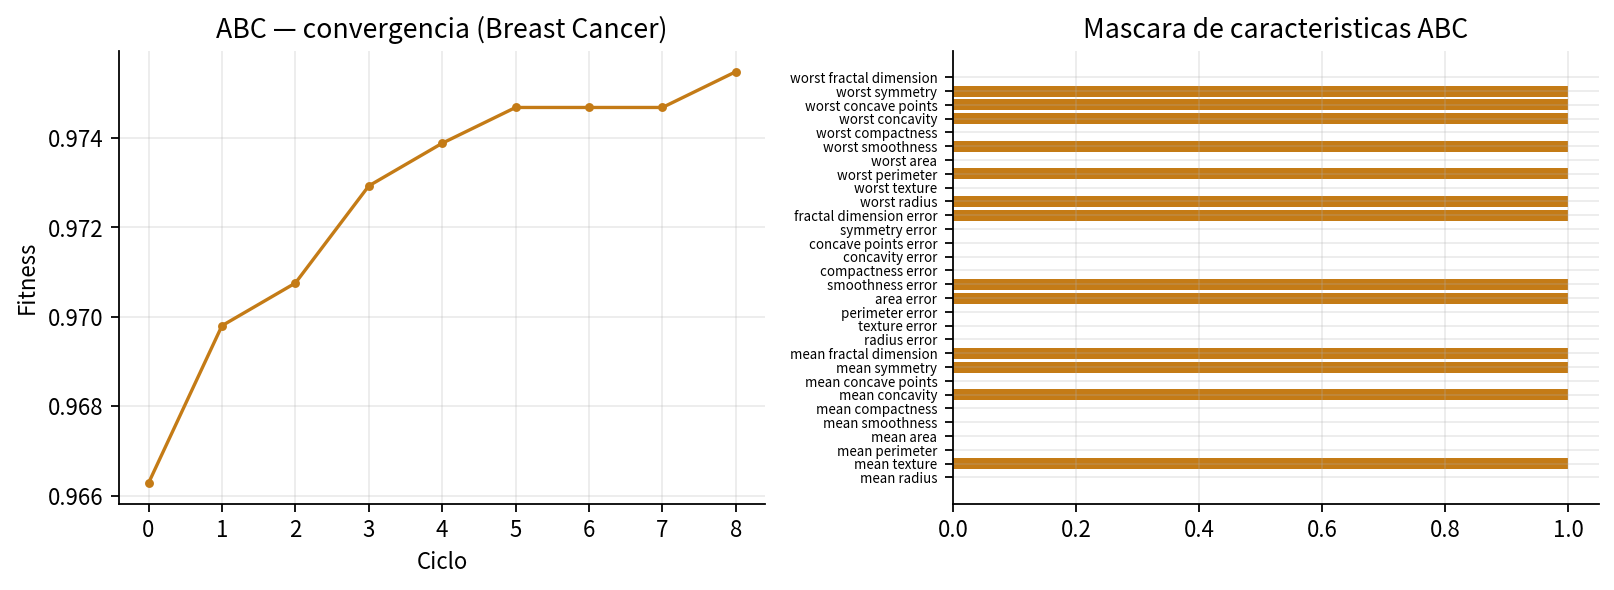
\includegraphics[width=0.96\textwidth]{../figures/01_abc_features.png}
\caption{Convergencia del fitness ABC y mascara binaria (Breast Cancer).}
\end{figure}
\begin{figure}[ht]\centering
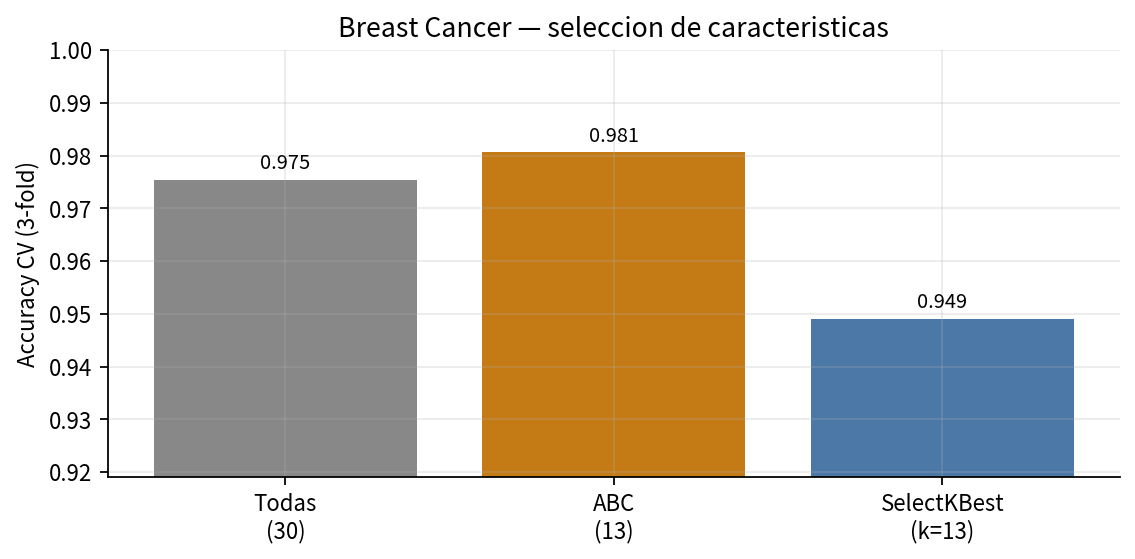
\includegraphics[width=0.78\textwidth]{../figures/01_abc_compare.png}
\caption{Comparacion de exactitud: todas las variables, ABC y SelectKBest.}
\end{figure}

\begin{cajagold}[Variables retenidas --- Breast Cancer]
\textit{mean texture, mean concavity, mean symmetry, mean fractal dimension, area error, smoothness error, fractal dimension error, worst radius, worst perimeter, worst smoothness, worst concavity, worst concave points, worst symmetry.}
\end{cajagold}

\subsection{Fragmento relevante}
\begin{lstlisting}[language=Python,caption={Vecindario binario y fitness wrapper.}]
def neighbor(src):
    k = rng.integers(0, n_bits)
    nxt = src.copy(); nxt[k] ^= 1
    if nxt.sum() == 0: nxt[k] = 1
    return nxt

def eval_mask(mask):
    if mask.sum() == 0: return 0.0
    acc = cross_val_score(clf, X[:, mask.astype(bool)], y, cv=cv).mean()
    return acc - 0.012 * (mask.sum() / mask.size)
\end{lstlisting}

\subsection{Discusion}
El termino de penalizacion evita la solucion trivial de usar todo. Limitacion: cada evaluacion reentrena el wrapper.

\section{Hyperparameter tuning con PSO}
\subsection{Problema}
Ajustar $C$ y $\gamma$ de un SVM RBF sobre Wine, en escala logaritmica.

\subsection{Ciclo del enjambre}
\begin{cajateal}[Ciclo PSO --- hiperparametros]
\textbf{Representacion.} $\mathbf{x}=(\log_{10}C,\;\log_{10}\gamma)\in[-2,3]\times[-4,1]$.\\[3pt]
\textbf{Inicializacion.} $10$ particulas uniformes.\\[3pt]
\textbf{Aptitud.} $J(C,\gamma)=1-\mathrm{Acc}_{CV}(\mathrm{SVM}_{RBF}(C,\gamma))$, 3-fold sobre el 70\% de entrenamiento.\\[3pt]
\textbf{Comportamiento.} PSO clasico, $w=0.7$, $c_1=c_2=1.5$.\\[3pt]
\textbf{Parada.} $10$ iteraciones ($110$ evaluaciones). Comparacion: Grid $5\times5$ y SVM por defecto.
\end{cajateal}

\subsection{Resultados}
PSO encontro $C\approx 92.3$, $\gamma\approx 0.0237$. Exactitud CV $0.992$; test $0.981$, por encima del grid ($0.963$).

\begin{table}[ht]
\centering
\caption{SVM-RBF en Wine. Test = 30\% estratificado.}
\begin{tabular}{lccc}
\toprule
\rowcolor{rowblue}
\textbf{Metodo} & Evals. & $C$, $\gamma$ & Acc.\ test \\
\midrule
SVM default & 1 & $1$, scale & 0.981 \\
Grid Search & 25 & $56.2$, $0.0316$ & 0.963 \\
PSO         & 110 & $92.3$, $0.0237$ & \textbf{0.981} \\
\bottomrule
\end{tabular}
\end{table}

\begin{figure}[ht]\centering
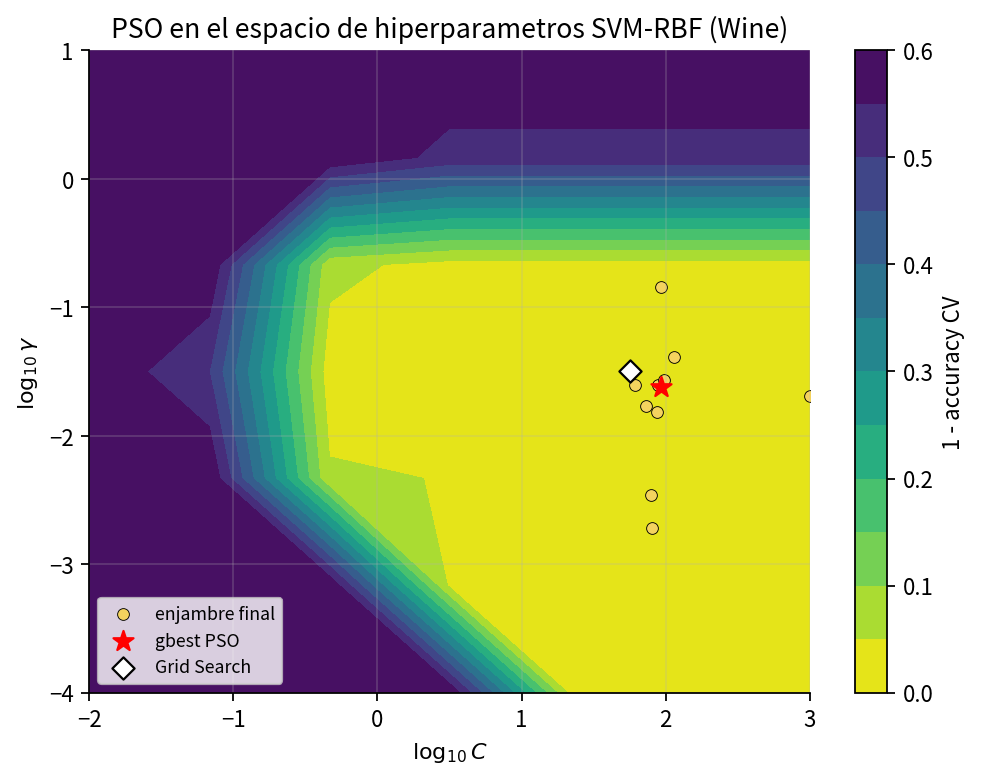
\includegraphics[width=0.70\textwidth]{../figures/02_pso_heatmap.png}
\caption{Paisaje de $1-\mathrm{Acc}_{CV}$. Estrella: gbest PSO. Rombo: grid.}
\end{figure}
\begin{figure}[ht]\centering
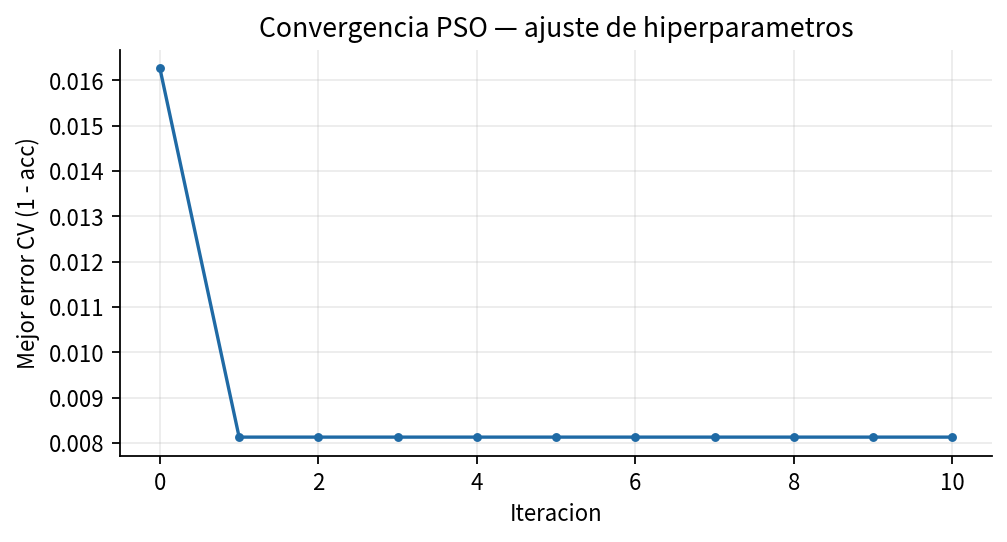
\includegraphics[width=0.80\textwidth]{../figures/02_pso_convergence.png}
\caption{Convergencia del mejor error de validacion cruzada.}
\end{figure}
\begin{figure}[ht]\centering
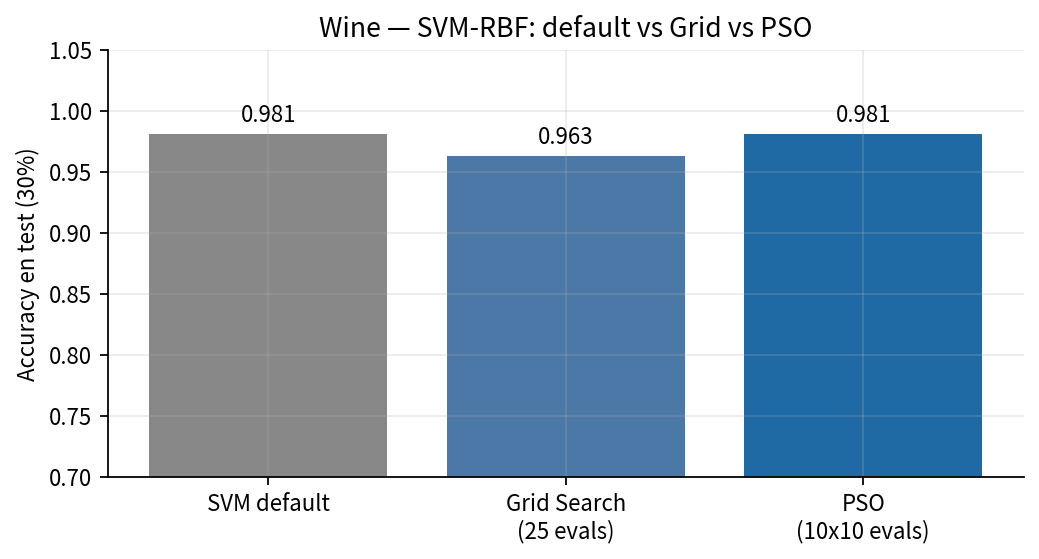
\includegraphics[width=0.76\textwidth]{../figures/02_pso_compare.png}
\caption{Exactitud de test: default, grid y PSO.}
\end{figure}

\subsection{Fragmento relevante}
\begin{lstlisting}[language=Python,caption={Particula PSO y funcion objetivo SVM.}]
def objective(p):
    C, g = 10**p[0], 10**p[1]
    acc = cross_val_score(SVC(C=C, gamma=g, kernel="rbf"),
                          Xtr, ytr, cv=inner).mean()
    return 1.0 - acc
\end{lstlisting}

\subsection{Discusion}
PSO no esta atado a una malla: se mueve en continuo y puede caer entre nodos del grid.

\section{Entrenamiento de una red neuronal sin backpropagation}
\subsection{Problema}
Red de \textbf{cuatro capas} $4$-$8$-$4$-$3$ sobre Iris, sin gradiente. Cada particula es una red completa ($91$ parametros). Apoyo visual: XOR con MLP $2$-$4$-$1$.

\subsection{Ciclo del enjambre}
\begin{cajateal}[Ciclo PSO --- pesos de la red]
\textbf{Representacion.} Vector $\mathbf{w}\in\mathbb{R}^{91}$.\\[3pt]
\textbf{Inicializacion.} $18$ particulas en $[-2.5,2.5]^{91}$.\\[3pt]
\textbf{Aptitud.} Entropia cruzada de entrenamiento. Solo hay \emph{forward}.\\[3pt]
\textbf{Comportamiento.} PSO con $w=0.65$, $c_1=c_2=1.6$.\\[3pt]
\textbf{Parada.} $25$ iteraciones. Comparacion: Adam, $400$ epocas.
\end{cajateal}

\subsection{Resultados}
PSO: CE $0.138$, train $0.943$, test $0.911$. Adam: test $0.756$. En XOR el MSE cayo a $8\cdot10^{-5}$.

\begin{table}[ht]
\centering
\caption{MLP $4$-$8$-$4$-$3$ en Iris (test 30\%).}
\begin{tabular}{lcc}
\toprule
\rowcolor{rowblue}
\textbf{Optimizador} & Parametros & Acc.\ test \\
\midrule
PSO (25 iter, 18 particulas) & 91 & \textbf{0.911} \\
Adam / backpropagation (400 epocas) & 91 & 0.756 \\
\bottomrule
\end{tabular}
\end{table}

\begin{figure}[ht]\centering
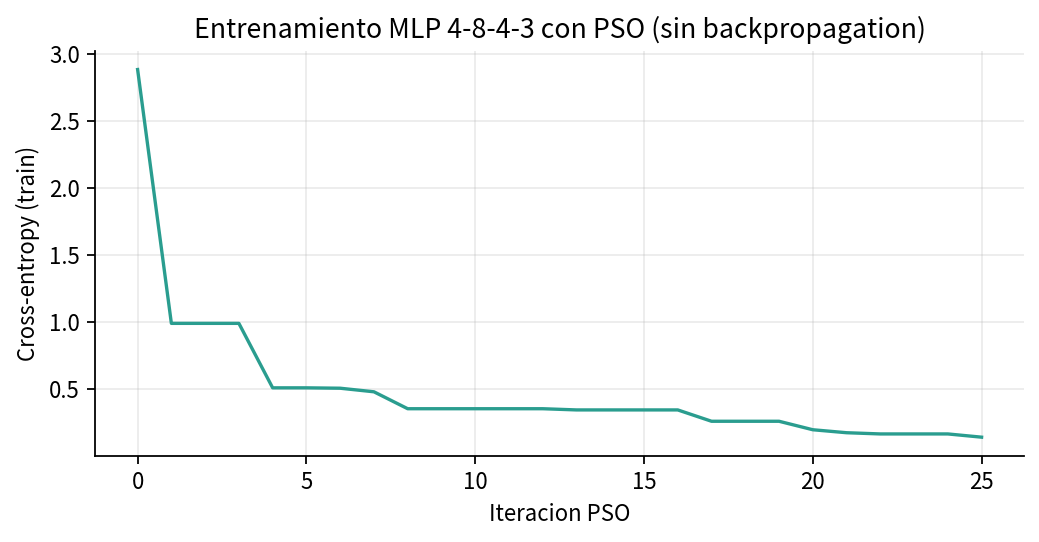
\includegraphics[width=0.80\textwidth]{../figures/03_nn_convergence.png}
\caption{Caida de la entropia cruzada (91 pesos movidos por el enjambre).}
\end{figure}
\begin{figure}[ht]\centering
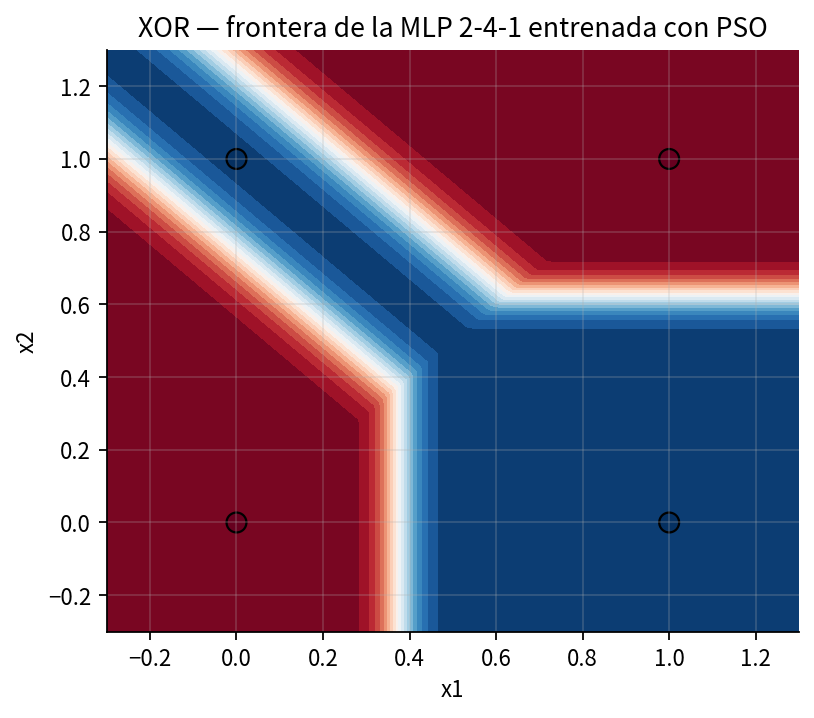
\includegraphics[width=0.60\textwidth]{../figures/03_xor_boundary.png}
\caption{Frontera de la MLP $2$-$4$-$1$ entrenada con PSO sobre XOR.}
\end{figure}
\begin{figure}[ht]\centering
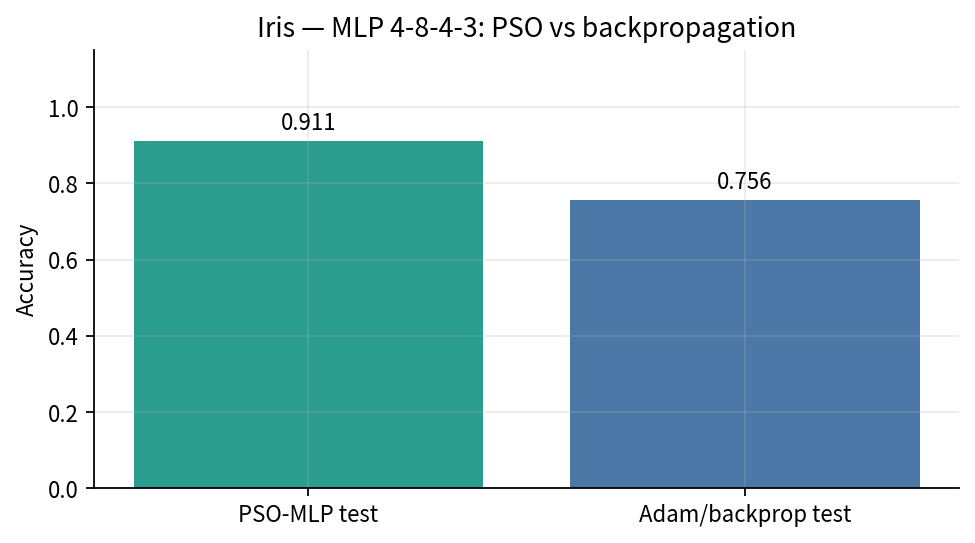
\includegraphics[width=0.70\textwidth]{../figures/03_nn_compare.png}
\caption{Exactitud de test: PSO versus Adam.}
\end{figure}

\subsection{Fragmento relevante}
\begin{lstlisting}[language=Python,caption={Forward sin backward.}]
def objective(w):
    pred = forward_mlp(Xtr, unpack(w, specs))
    return -np.mean(np.log(pred[np.arange(len(ytr)), ytr] + 1e-8))
\end{lstlisting}

\subsection{Discusion}
PSO no escala a redes enormes. El valor didactico es mostrar que backpropagation es un optimizador, no la definicion de aprender.

\section{Clustering con PSO}
\subsection{Problema}
Hallar $K$ centroides que minimicen la inercia. \texttt{make\_blobs} ($n=360$, $K=4$) y Wine en 2 variables ($K=3$).

\subsection{Ciclo del enjambre}
\begin{cajateal}[Ciclo PSO --- clustering]
\textbf{Representacion.} $\mathbf{x}=(\mathbf{c}_1\|\cdots\|\mathbf{c}_K)\in\mathbb{R}^{Kd}$.\\[3pt]
\textbf{Inicializacion.} $18$ particulas dentro del rango de $X$.\\[3pt]
\textbf{Aptitud.} Suma de distancias al cuadrado al centroide mas cercano.\\[3pt]
\textbf{Comportamiento.} Cada particula mueve todos los centroides.\\[3pt]
\textbf{Parada.} $22$ iteraciones. Baseline: K-Means \texttt{n\_init=10}.
\end{cajateal}

\subsection{Resultados}
En blobs, K-Means gana (inercia $504$ vs $2407$, silueta $0.824$ vs $0.610$). En Wine-2D empatan en $0.484$. El resultado es util porque no es un empate automatico.

\begin{table}[ht]
\centering
\caption{Clustering: PSO versus K-Means.}
\begin{tabular}{lcccc}
\toprule
\rowcolor{rowblue}
\textbf{Datos} & Inercia PSO & Inercia KM & Sil.\ PSO & Sil.\ KM \\
\midrule
Blobs $K=4$ & 2407 & \textbf{504} & 0.610 & \textbf{0.824} \\
Wine-2D $K=3$ & --- & --- & 0.484 & 0.484 \\
\bottomrule
\end{tabular}
\end{table}

\begin{figure}[ht]\centering
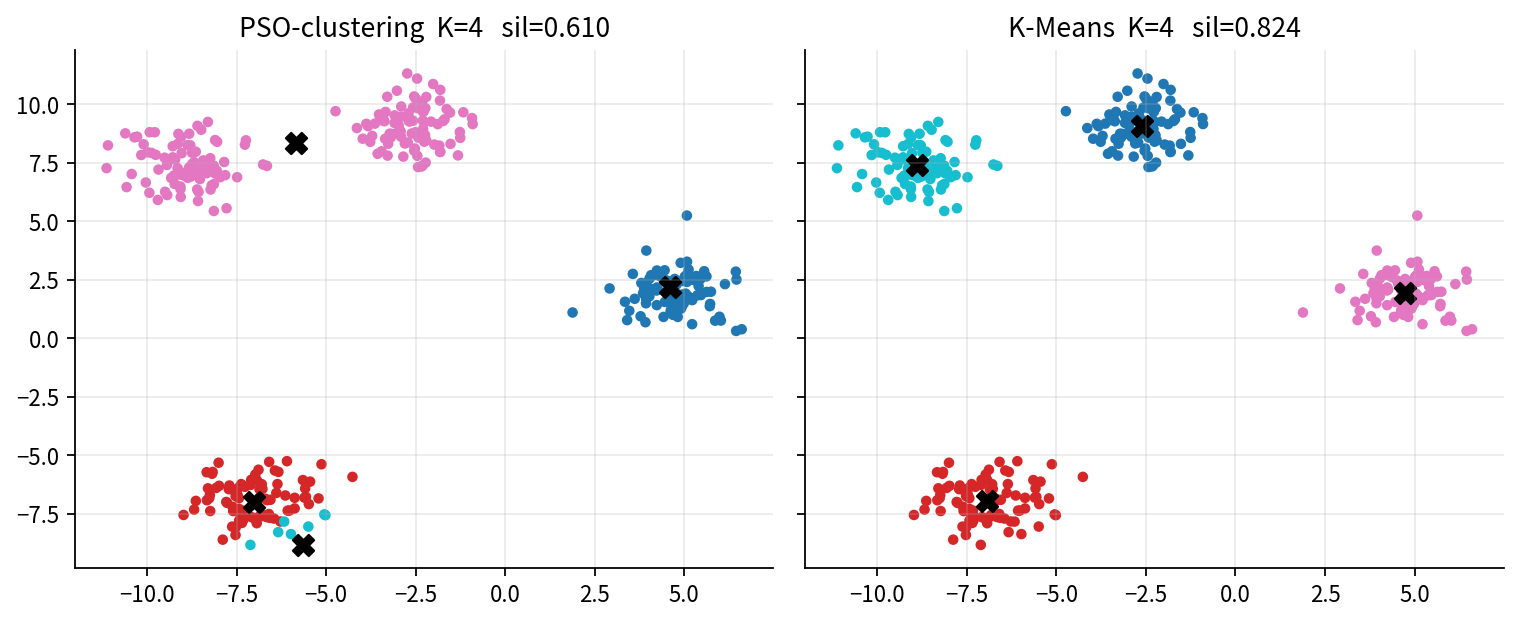
\includegraphics[width=0.94\textwidth]{../figures/04_clusters.png}
\caption{Particiones y centroides de PSO y K-Means sobre blobs.}
\end{figure}
\begin{figure}[ht]\centering
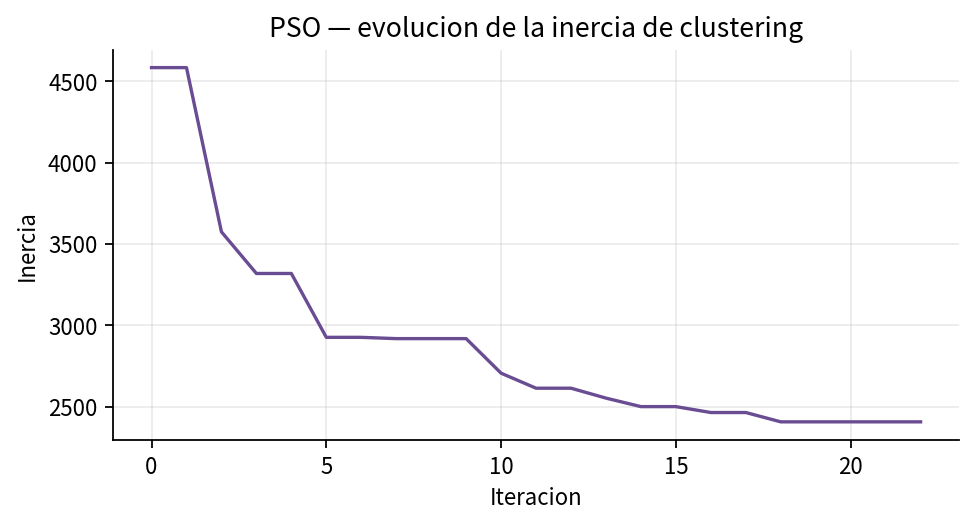
\includegraphics[width=0.76\textwidth]{../figures/04_cluster_convergence.png}
\caption{Evolucion de la inercia del mejor individuo.}
\end{figure}
\begin{figure}[ht]\centering
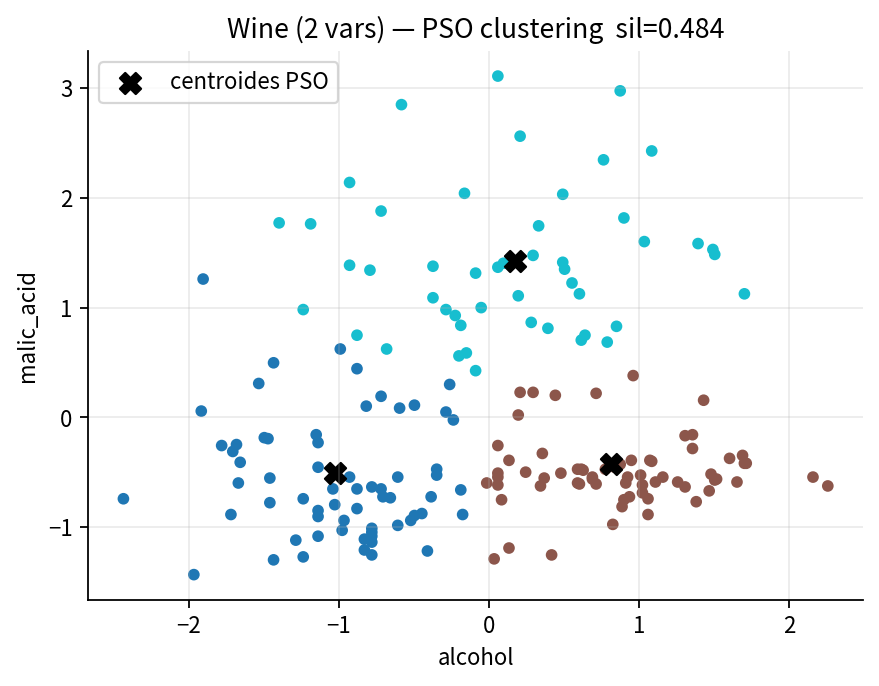
\includegraphics[width=0.60\textwidth]{../figures/04_wine_clusters.png}
\caption{PSO-clustering sobre las dos primeras variables de Wine.}
\end{figure}

\subsection{Fragmento relevante}
\begin{lstlisting}[language=Python,caption={Particula = K centroides concatenados.}]
def inertia(pos):
    C = pos.reshape(K, 2)
    d = ((X[:, None, :] - C[None, :, :])**2).sum(axis=2)
    return d.min(axis=1).sum()
\end{lstlisting}

\section{Reproducibilidad y repositorio}
Ambiente: Python 3, \texttt{numpy}, \texttt{scikit-learn}, \texttt{matplotlib}. Semilla $42$.
\begin{lstlisting}[language=bash]
python src/experiments.py
\end{lstlisting}
\begin{cajarepo}
\url{https://github.com/paololuna-luw/algoritmos-enjambre}\\[6pt]
\texttt{README.md} \quad \texttt{requirements.txt} \quad \texttt{src/experiments.py}\\
\texttt{figures/} \quad \texttt{report/informe.tex} \quad \texttt{report/informe.pdf}
\end{cajarepo}

\section{Conclusiones}
\begin{enumerate}[leftmargin=1.4em]
  \item ABC reduce variables y mejora exactitud frente al vector completo y a SelectKBest.
  \item PSO recorre el plano $(\log C,\log\gamma)$ y localiza un SVM competitivo.
  \item Una MLP de cuatro capas se puede entrenar solo con forward + PSO.
  \item El mismo PSO formula clustering como optimizacion de centroides; K-Means sigue siendo mas eficiente aqui.
  \item Los cuatro ejemplos comparten el mismo ciclo, que es el objeto de la actividad.
\end{enumerate}

\begin{thebibliography}{9}
\bibitem{karaboga2005} D.~Karaboga. \emph{An idea based on honey bee swarm for numerical optimization}. TR06, Erciyes University, 2005.
\bibitem{kennedy1995} J.~Kennedy and R.~Eberhart. Particle swarm optimization. In \emph{Proc.\ ICNN}, 1995.
\bibitem{schiezaro2013} M.~Schiezaro and H.~Pedrini. Data feature selection based on Artificial Bee Colony algorithm. \emph{EURASIP J.\ Image Video Process.}, 2013.
\end{thebibliography}
\end{document}
